\documentclass[10pt,twocolumn]{article}
\usepackage[margin=0.85in]{geometry}
\usepackage{graphicx}
\usepackage{booktabs}
\usepackage{amsmath,amssymb}
\usepackage[numbers]{natbib}
\usepackage[hidelinks]{hyperref}
\usepackage{stfloats}
\usepackage{caption}
\graphicspath{{../}}
\raggedbottom
\renewcommand{\topfraction}{0.95}
\renewcommand{\textfraction}{0.05}
\renewcommand{\floatpagefraction}{0.85}

\title{\textbf{\Large Self-Knowledge Does Not Scale}\\[3pt]
\normalsize A capability-invariant floor on language-model introspection}
\author{David Condrey \\ \small WritersLogic, Inc. \\ \small \texttt{david@writerslogic.com}}
\date{}

\begin{document}
\twocolumn[
\begin{@twocolumnfalse}
\maketitle
\vspace{0.4em}
\end{@twocolumnfalse}
]

\begin{abstract}
\noindent A language model's ability to report on its own state does not improve with capability. Across a
144x parameter range (0.5B to 72B) and three model families, a model's stated probability of its own answer
stays about 0.3 from its actual answer distribution, and the correlation between the two plateaus near 0.65
rather than approaching accurate self-report; the tenfold step from 7B to 72B buys nothing. Interpretability
and safety increasingly treat self-report as a window into the model that sharpens as models improve; we
find instead a floor that neither scale nor training recipe lowers. The gap is genuine self-knowledge, not
generic miscalibration: capable models predict their own answers reliably better than a generic peer's, but
this privileged self-access is thin (about 0.1) and flat across scale. The failure is positive, not an
absence: models report confident-looking probabilities that are systematically wrong about their own
decisive behavior. Self-transparency is not something a model scales into, which bears on oversight that
relies on models reporting their own states.
\end{abstract}

\section{Introduction}
A growing set of interpretability and oversight methods asks the model itself: how confident are you, what
are you attending to, would you answer the same way again. The implicit bet is that self-report is a window
into the model, and that the window sharpens as models get more capable. We test that bet and find it
false. A model's report about its own state does not converge on its actual state as capability grows; it
saturates early at a substantial error and stays there.

Concretely, we compare two quantities on the same questions: what a model \emph{does}---its answer
distribution, read from token logprobs---and what it \emph{says} it does---a probability it reports about
its own answer. A model that could read its own state would make these agree. Instead the stated and actual
probabilities differ by about 0.3 on average, and this gap does not shrink from 0.5B to 72B parameters, nor
across the Qwen2.5, Yi-1.5, and Falcon3 families. The picture is vivid (Fig.~\ref{fig:scatter}): a capable
model answers decisively---actual $P(\text{Yes})$ at 0 or 1---while reporting moderate confidence near 0.5.
It behaves as if certain and reports as if unsure.

Our contribution is the missing empirical axis. Introspective opacity is not new: attention-schema theory
holds that reports draw on a schematic, mechanism-blind self-model \citep{webb2015}, and the meta-problem
frames the opacity directly \citep{chalmers2018}. What no prior account supplies is how opacity behaves as a
function of capability. We supply it and find the opacity is \emph{capability-invariant}. We further show,
with a self-versus-peer control, that the gap is genuinely about self-knowledge and not generic
miscalibration: capable models predict their own answers reliably better than a stranger's---but this
privileged self-access is thin (about 0.1) and, like the gap itself, flat across scale. Self-report is a
floored guess, not a window that clears with capability.

\section{Related work}
\textbf{Introspective opacity is predicted, but not its scaling.} Attention-schema theory \citep{webb2015,
wilterson2021} explains why a system's self-report can be systematically wrong: the self-model is a
schematic caricature of the underlying mechanism. The meta-problem \citep{chalmers2018} makes the opacity
its subject. These are qualitative and architecture-level; none asks whether the opacity is a fixed
feature, a trainable deficit, or a capability-invariant floor. That empirical question is ours.

\textbf{Calibration treats it as trainable.} A large literature elicits verbalized confidence and finds it
poorly calibrated \citep{kadavath2022}, and treats the fix as a training problem. Calibration to
correctness is not our target: our questions are largely subjective, and we score the self-report against
the model's \emph{own} behavior, not against truth. We measure whether a model can read its own answer
distribution, and whether that ability grows with scale; it does not.

\textbf{Introspective self-report, measured.} \citet{binder2025} show models can learn limited behavioral
self-prediction; \citet{anthropic2025} measure introspective reports as unreliable and sometimes
confabulated; \citet{premakumar2024} treat self-modeling as regularization. We give a mechanism-agnostic,
scale-resolved measurement and a positive characterization---a thin, capability-invariant self-access.

\textbf{Physical precedent.} That self-measurement can be irreducibly limited is old: an observer contained
in a system cannot accurately measure that system's state \citep{breuer1995}. A companion study measures
this floor physically, on real hardware; it motivates asking whether computational self-report is similarly
floored, which we here find it is. We draw the analogy but do not claim the mechanisms are identical.

\section{Measuring what a model says against what it does}
\textbf{Behavior.} For a yes/no question $q$ we prompt the model to answer with a single word and read the
first-token probabilities of \texttt{Yes} and \texttt{No}, giving the actual answer distribution
$b = P(\text{Yes})$. \textbf{Self-report.} Separately we ask the model, in words, for the probability that
it would answer Yes, and parse an integer 0--100, giving the stated $s$. \textbf{Gap and correlation.} The
introspective gap on $q$ is $|s-b|$; across items we also report the rank correlation between $s$ and $b$.
A model with accurate self-knowledge has gap $0$ and correlation $1$.

\textbf{Self versus peer.} To separate self-knowledge from generic miscalibration we also ask the model to
predict a \emph{generic, unrelated} assistant's answer, giving $o$, and score both against the model's own
behavior: $\text{gap}_{\text{self}}=|s-b|$, $\text{gap}_{\text{other}}=|o-b|$. The self advantage
$\text{gap}_{\text{other}}-\text{gap}_{\text{self}}$ is positive only if the model reads itself better than
it reads a stranger.

\textbf{Items and models.} We use 38 binary questions spanning ambiguous, subjective, and borderline-factual
prompts; all decoding is greedy. We sweep Qwen2.5-Instruct at 0.5, 1.5, 3, 7, 14, 32, and 72B, and replicate
across families with Yi-1.5 (6, 9, 34B) and Falcon3 (7, 10B). Confidence intervals are 2000-sample
bootstraps. Code and per-model outputs are released (\S\ref{sec:repro}).

\begin{figure*}[t]
\centering
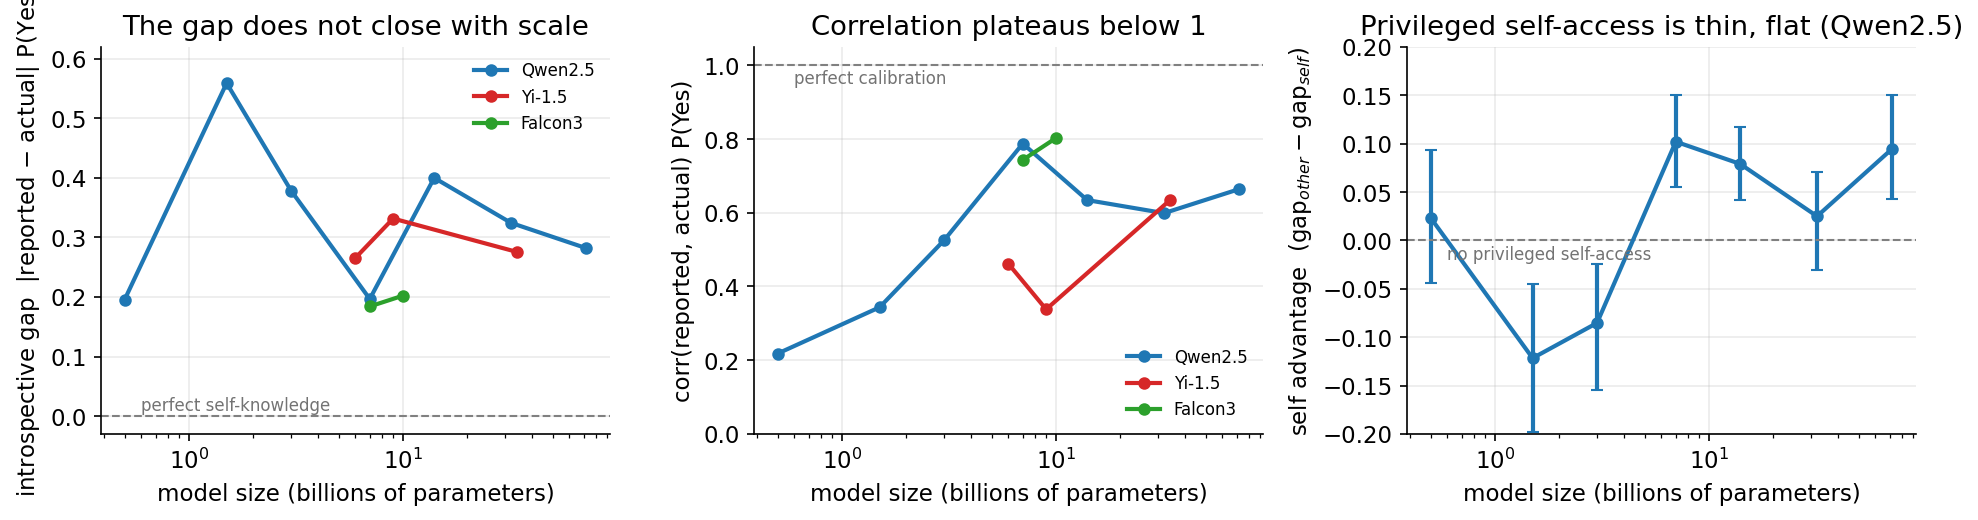
\includegraphics[width=0.97\textwidth]{fig6_introspection_scale.png}
\caption{Introspective self-knowledge is capability-invariant. \textbf{Left:} the gap between stated and
actual $P(\text{Yes})$ stays near 0.3 and never falls toward zero. \textbf{Center:} the correlation between
stated and actual self-report plateaus below 1---the tenfold step from 7B to 72B does not improve it.
\textbf{Right:} a model predicts its own answer only marginally better than a generic peer's (self
advantage), and that thin advantage neither grows with scale nor closes the gap. Error bars are 95\%
bootstrap CIs; three families shown.}
\label{fig:introscale}
\end{figure*}

\section{Self-knowledge does not scale}
The introspective gap does not close and self-report does not become calibrated as models grow
(Fig.~\ref{fig:introscale}, Table~\ref{tab:scale}). Within Qwen2.5, capability helps only up to about 7B:
the gap falls and the correlation rises through the small models, then flattens. From 7B to 72B---a tenfold
increase in parameters---the correlation sits near 0.65 and the gap near 0.3, with no trend toward accurate
self-report. The largest model we test reads its own answer distribution no better than a mid-size one.

The pattern is not an artifact of one training recipe. Yi-1.5 reproduces the plateau across 6B to 34B, and
Falcon3, though better calibrated in absolute terms (gap $\approx 0.2$), still does not close it. No model
among the twelve tested, across three families and a 144x parameter range, achieves accurate self-report,
and the residual is flat in scale.

\begin{table}[t]
\centering
\small\setlength{\tabcolsep}{5pt}
\begin{tabular}{llcc}
\toprule
family & size & gap & corr \\
\midrule
Qwen2.5 & 0.5B & 0.20 & 0.22 \\
Qwen2.5 & 1.5B & 0.56 & 0.34 \\
Qwen2.5 & 3B   & 0.38 & 0.53 \\
Qwen2.5 & 7B   & 0.20 & 0.79 \\
Qwen2.5 & 14B  & 0.40 & 0.64 \\
Qwen2.5 & 32B  & 0.32 & 0.60 \\
Qwen2.5 & 72B  & 0.28 & 0.66 \\
\midrule
Yi-1.5   & 6B   & 0.27 & 0.46 \\
Yi-1.5   & 9B   & 0.33 & 0.34 \\
Yi-1.5   & 34B  & 0.28 & 0.63 \\
Falcon3  & 7B   & 0.18 & 0.74 \\
Falcon3  & 10B  & 0.20 & 0.80 \\
\bottomrule
\end{tabular}
\caption{Introspective gap ($|$stated$-$actual$|$ $P(\text{Yes})$, lower is better) and rank correlation
between stated and actual self-report (higher is better) across model scale and family. No model closes the
gap; correlation never approaches 1.}
\label{tab:scale}
\end{table}

The failure is concrete and positive (Fig.~\ref{fig:scatter}). A capable model's behavior is pinned at 0 or
1---it answers decisively---while its self-report clusters near 0.5. It states a confident-looking number
that is systematically wrong about how decisive it actually is. This is a misrepresentation the model
positively makes, not merely a self-fact it fails to represent.

\begin{figure}[t]
\centering
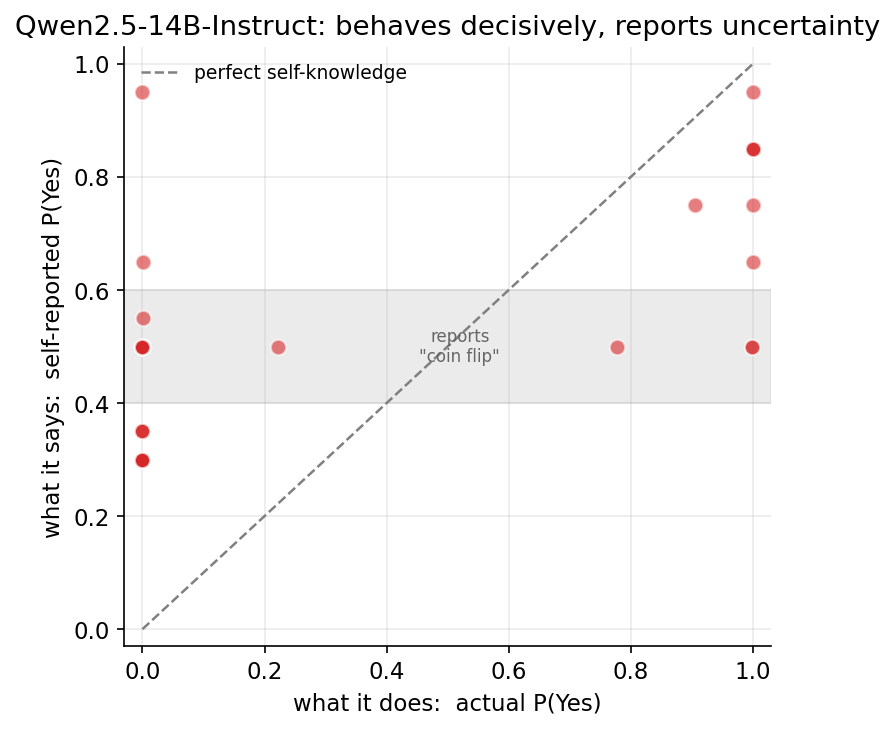
\includegraphics[width=\columnwidth]{fig7_calibration_scatter.png}
\caption{Per-question stated versus actual $P(\text{Yes})$ for one model (Qwen2.5-14B). Behavior is pinned
at 0 or 1; the self-report clusters near 0.5. The model behaves decisively and reports uncertainty; points
sit far from the diagonal of accurate self-knowledge.}
\label{fig:scatter}
\end{figure}

\section{The gap is self-specific, but the self-access is thin}
A natural objection is that this is generic miscalibration---models are simply bad at stating probabilities
about anything, self or not. It is not. When we ask a model to predict a generic peer's answer and score
both predictions against its own behavior, the capable models predict themselves reliably better than the
peer: at 7B, 14B, and 72B the self advantage is $+0.10$, $+0.08$, and $+0.10$, each with a 95\% CI excluding
zero (Fig.~\ref{fig:introscale}, right). There is genuine self-specific information in the self-report.

But the privileged window is narrow. The advantage is only about $0.1$ while the self-prediction error
itself stays near $0.3$; knowing it is ``you'' closes barely a quarter of the gap, and the advantage is
flat across the 144x range. A model's self-model is largely a model of a generic agent, with a thin,
capability-invariant layer of true self-access on top. It reads its own state a little better than a
stranger's, and nowhere near well enough to recover it.

\section{Implications}
If self-report were a window that sharpened with capability, waiting for better models would eventually make
introspective oversight reliable. It does not sharpen. Oversight and interpretability methods that ask a
model to report its own confidence, attention, or reasoning are reading a floored, mostly-generic self-model,
and scale will not fix this for them. The result is not that self-report is useless---the thin self-specific
layer is real and could be leveraged---but that it must be treated as a weak, capped signal, not a window
that clears. It also reframes introspective opacity: attention-schema accounts explain why the self-model is
schematic; we add that its schematic-ness is capability-invariant, a property of the systems, not a stage
they grow out of.

\section{Limitations}
We state these plainly. (1) Self-report is elicited as a verbalized probability; a verbalized probability and
a token-level probability are different readouts, and part of the gap may reflect that mismatch---though the
positive self-versus-peer advantage shows the report carries real self-information, not just channel noise.
(2) 38 items, greedy decoding, one elicitation template per condition; we have not swept prompt phrasings or
sampling temperature. (3) The gap's magnitude is family-dependent (Falcon3 is better calibrated), so the
claim is qualitative---a non-closing floor---not a universal constant. (4) The scale evidence is strongest in
Qwen2.5 (144x) and Yi-1.5; the largest models are read in 4-bit. (5) We measure answer-distribution
self-report; other internal states may behave differently. None of these is closed by more capability, which
is the point.

\section{Conclusion}
A language model does not read its own state better as it grows more capable. Across 144x of scale and three
families, the gap between what a model does and what it says it does stays near 0.3, correlation plateaus
below accurate self-report, and the genuinely self-specific part of the report is thin and flat.
Self-transparency is not a capability a model scales into; it is a floor. Systems built on the assumption
that better models will introspect more reliably are building on that floor.

\paragraph{Reproducibility.}\label{sec:repro} All code, per-model results, and figure scripts are at
\url{https://github.com/dcondrey/cost-of-self-knowledge}: \texttt{introspect\_calibration.py} (gap and
scale), \texttt{introspect\_selfspecific.py} (self versus peer), \texttt{modal\_introspect.py} (the sweep
harness), and \texttt{make\_introspect\_figs.py}, with all \texttt{results/*.json}.

\bibliographystyle{plainnat}
\bibliography{refs}
\end{document}
